\section{CityScope Volpe}\label{sec:cityscope_volpe}
{
    \subsection{Introduction}

    {
        Building upon the PlayGround-TRP project \eqref{sec:cityscope_playground}, this work extends CityScope with different layers of information and real-time analytics. The urban context for this project was the Volpe site in Cambridge, MA, which in 2016, was still vacant and set for redevelopment. CityScope Volpe was designed to explore the impact of different interventions, both within the site and its surrounding context, with three primary objectives: (i) To communicate complex urban data and the inter-relationships between urban systems; (ii) To simulate the impact of urban interventions; (iii) To support decision making in an iterative process using a tangible interface. Figure \eqref{fig:volpe_overall} shows CityScope Volpe, the TUI, and the real-time metrics.
    }

    \begin{figure}[!htb]
        \begin{center}
            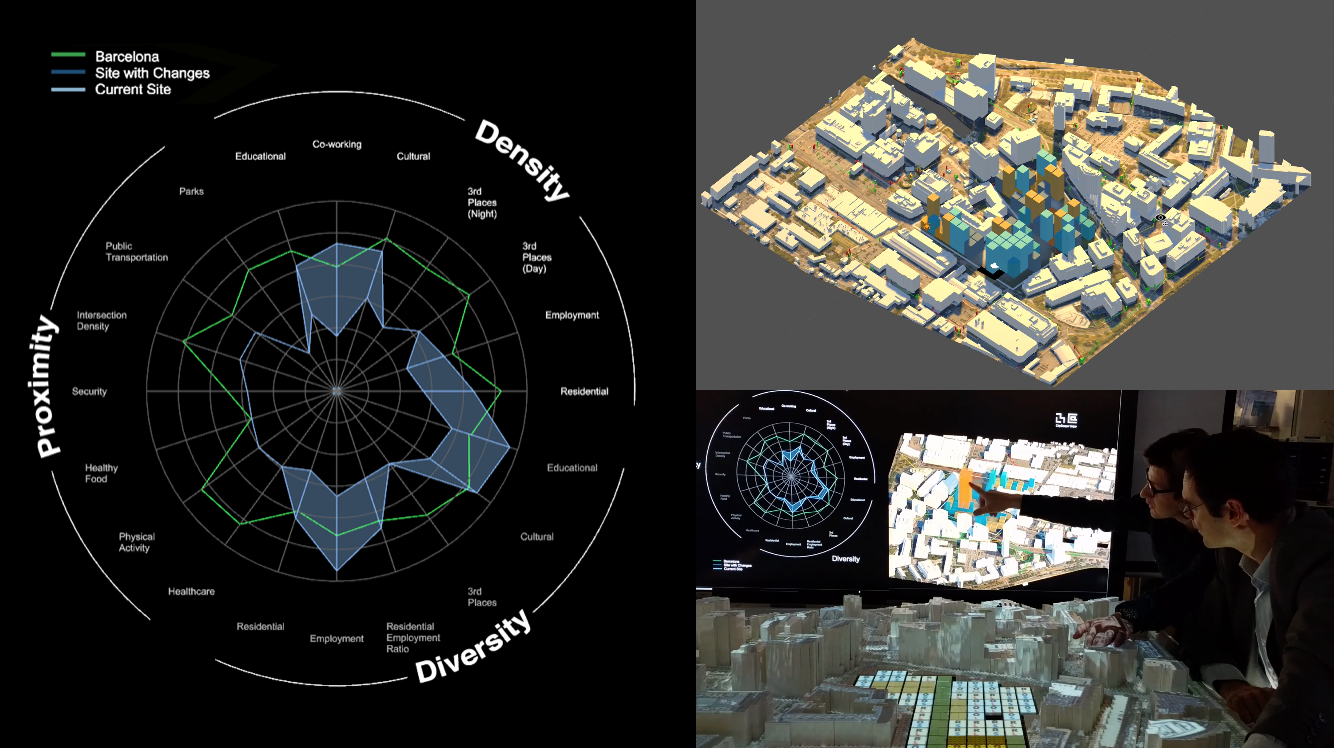
\includegraphics[width=1\linewidth]{chapters/transformation/volpe/figures/volpe0.png}
        \end{center}
        \caption{CityScope Volpe. (left) a set of KPIs and urban indicators are evaluated with each design iteration. (upper-right) The users interactions are translated to three-dimensional zoning envelops, which represent the maximal intervention framework, rather than actual building volumes. (lower-right) Users are presented with both outputs as a mean to direct their design collaboration process.}
        \label{fig:volpe_overall}
    \end{figure}

    \subsection{Site and context}
    {
        As discussed in the previous project \eqref{appendix:playground}, Kendall Sq. was going through extreme urban transformation, driven by the proximity to MIT, Harvard, and the many industries in this area. A limited housing stock and high land values made most residential opportunities in the area out of reach: With a residential density of $\sim$3,000/km$^2$, most workers commute long distances from the greater Boston area, at the cost of energy and time \cite{blanding_blanding_2016}. Additionally, affordable housing incentives were inadequately promoting the necessary range of housing options, and the zoning ordinance has overly restrictive land-use requirements \cite{noyman2015powerstructures}. Alongside low residential density, is the scarcity of services, amenities and 3rd-places, which tend to indicate the urban vitality of a place \cite{Glaeser2011, banerjee2011companion}.
    }

    \subsection{Method} \label{subsec:vople_cityscope}

    {
        CityScope Volpe was built to investigate the redevelopment of the 14-acre DOT facility site, purchased by MIT in 2019 \cite{mit_news}. The physical 3D model is built using LEGO and covers a region of $1km^2$ at a scale of 1:762m\footnote{each 4x4 LEGO tile represents a 26.7 x 26.7 meter area, or 6.675m per LEGO stud.}. Similar to the TRP \eqref{sec:cityscope_playground}, the interactive portion of the model is integrated into the surroundings to represent the area under development, as shown in Figure \eqref{fig:volpe_site}. This intervention region utilizes `CityMatrix' \cite{zhang2017citymatrix}, a Rhino-Grasshopper script \cite{TheHisto40:online} for scanning and virtually reconstructing the interactive site. Interchangeable LEGO tiles represent different land-uses ranging from roads, parks, amenities, residential or office buildings. The TUI also includes physical components with sliders and toggles to change the building height and switch between alternative mobility modes. These modifications are recorded and passed to the computational analysis unit in order to provide real-time feedback to the user. The next section describes the different metric computed by the platform, and the different auxiliary tools and software used to compute them.
    }


    \begin{figure}[!htb]
        \begin{center}
            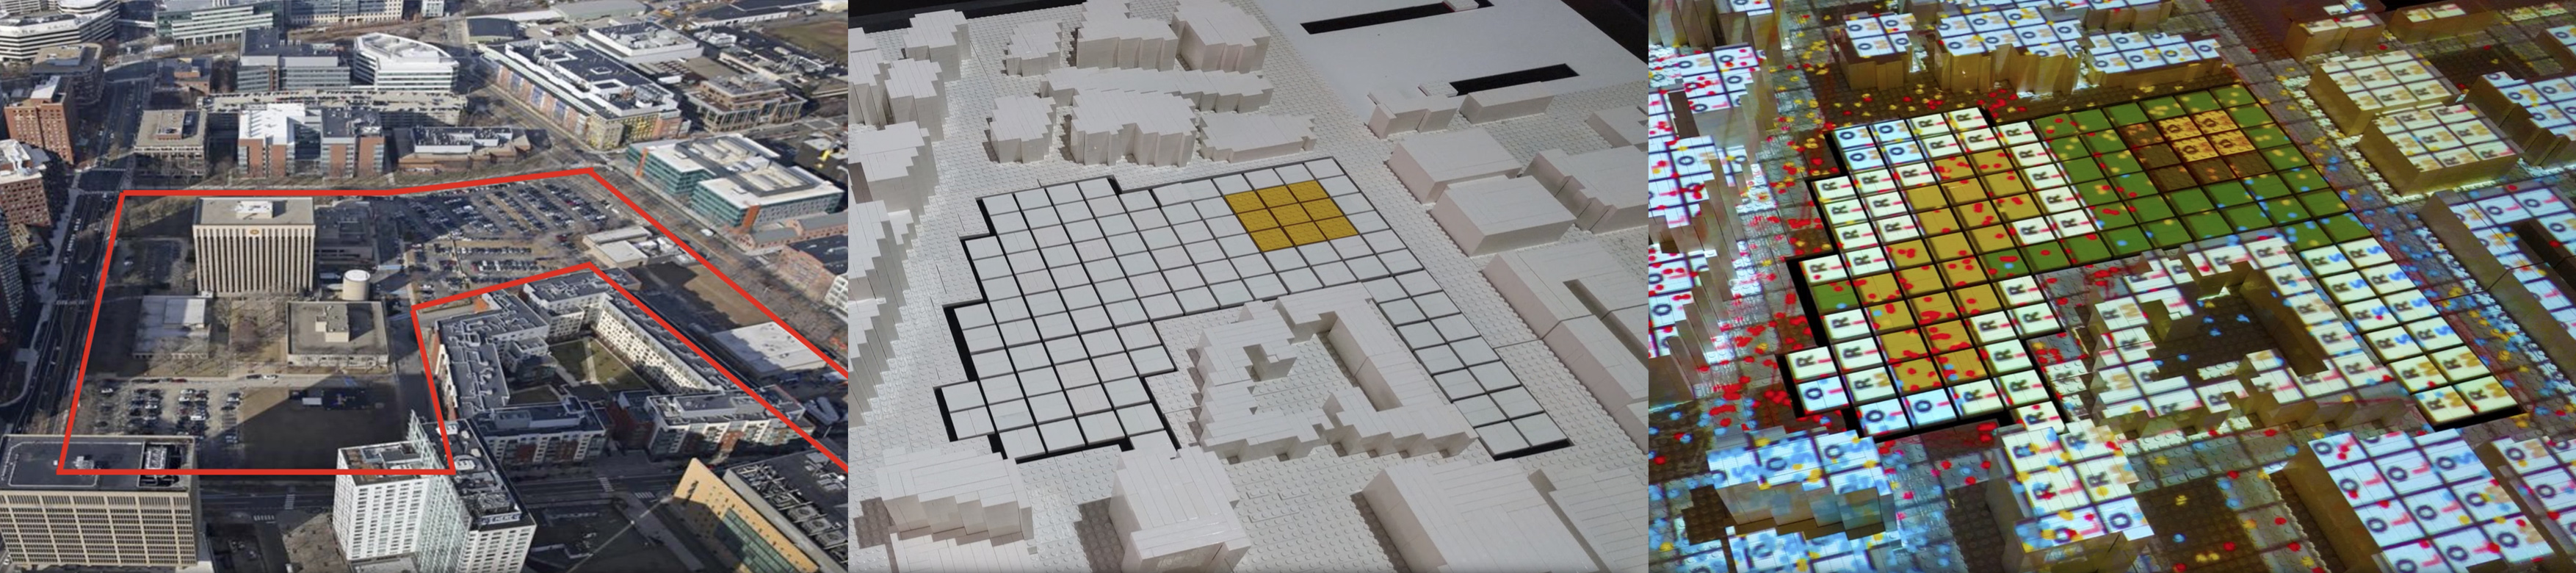
\includegraphics[width=1\linewidth]{chapters/transformation/volpe/figures/volpe3.jpg}
        \end{center}
        \caption{The DOT Volpe facility site. The redevelopment site is abstracted to the CityScope grid, in which the context is immutable and the site is interactive.}
        \label{fig:volpe_site}
    \end{figure}

    \subsection{Urban Performance Indicators}

    {
        In CityScope Volpe, urban performance is analyzed in terms of social, economic and physical attributes, which are clustered as Density, Diversity, Proximity, Mobility, Building Energy and Innovation Potential \cite{katz2014rise}. The computational analysis uses a number of tools to calculate a range of performance metrics, and produces feedback in the form of both spatial and numerical statistics, including Rhino-Grasshopper, GAMA platform, and Unity \cite{TheHisto40:online, grignard2013gama, UnityRea35:online, noyman2018CityScopeARUD}. The different urban performance indicators are shown in Figure \eqref{fig:volpe_overall}. The rest of this section overviews the different metrics and indicators used in the analysis.

        \subsubsection{Density}
        {
            The ratio between housing, commercial space, retail venues, cultural institutions, and other amenities is known to be related to the creation of well functioning cities \cite{lynch1984good, gehl2013study, katz2014rise}. Density has to be balanced in order to ensure positive outcomes (such as greater exchange of ideas, economic mobility, more employment options, better amenities, or energy reduction) with fewer negative outcomes (such as traffic congestion, lack of natural resources, or pollution) \cite{hawley1972population, UnitedNationsHabitatIII2017, deloitte_2021}. In Volpe, the density of each land-use type (eg. amenities, residences, employment) can be represented as $Density^m=\frac{|M|}{A}$, where $M$ is the set of occurrences of $m$ in the design area, and $A$ is the total area of district.
        }


        \begin{figure}[!htb]
            \begin{center}
                \includegraphics[width=1\linewidth]{chapters/transformation/volpe/figures/volpe2.png}
            \end{center}
            \caption{User interaction and feedback. As users interact with the CityScope TUI, urban performance indicators update in real-time: density, diversity, proximity, mobility energy per person, walkability, access to parks, and a simulated probability of meeting areas (so called `collision potential').}
            \label{fig:volpe_layers}
        \end{figure}

        \subsubsection{Diversity}
        {
            Highly performative urban areas tend to present an increased diversity of social, economic and spatial characteristics. The Diversity index is assessed using a Shannon-Weaver formula \cite{kemeny2013immigrant} and Balanced Ecosystem index: Quantitative measurement that reflects how many different types (species) there are in a certain set (community/ecosystem), and simultaneously takes into account how evenly the basic entities (individuals) are distributed among those types. This can be represented as $H = - \displaystyle\sum_{i=1}^{S} p_i ln p_i$, where $H$ is the Shannon diversity index, $S$ is the total number of species in the community, and $p_i$ is the proportion of the population made up of species $i$. Naturally, not all species are - or should be - equally represented, and the diversity index only measures the distribution of these species.
        }

        \subsubsection{Proximity}

        {
            Proximity assesses the accessibility and closeness indexes between social, economic and physical functions in urban environments \cite{sevtsuk2016pedestrian}. Historically, high performing cities resemble networks of compact urban districts where resources and amenities of daily life are in close proximity to one another \cite{westerink2013dealing}. In Volpe, proximity metrics include walkable access to parks, housing, jobs, mass transit, schools, and amenities. For a given `goal object', a proximity metric for a district can be calculated as $Closeness\,to\,SM = (\sum\limits_{j\epsilon B_i} dist(j,closest(j,SM)))^{-1}$, where $B_i$ is the set of tiles in district $i$, $SM$ is the `goal' objects (Parks, Residential, Office, etc.), $dist (a; b)$ is the geographical distance between two elements' centroids $a$ and $b$, and $closest (j;Y)$ is geographically closest element in set $Y$ from block $j$ centroid. Figure \eqref{fig:volpe_layers}(top) shows the proximity metric for parks in the Volpe site as a heatmap over TUI.
        }

        \subsubsection{Mobility Energy}
        {
            Several mobility metrics are introduced in this project. An Agent Based Model (ABM) simulates a synthetic population in response to changes in land-use and mobility modes, and calculates the energy produces by each trip \cite{grignard2017agent}. The impacts of urban mobility on energy consumption can be calculated as $E_m = \sum_{m \in M}\sum_{l \in L}v_l^m s_{l} e^m$ where $E_m$ is the total mobility energy, $M, L$ is the set of all transport modes and road network links respectively, $v_l^m$ is the number of vehicles of mode $m$ that travel on link $l$, $s_l$ is the length of link $l$, and $e_m$ is the energy usage per unit distance traveled by mode $m$.
        }

        \subsubsection{Building Energy}
        {
            Energy Consumption is calculated for structures in and around the Volpe area using building envelope performance data, orientation, estimated embodied energy, and land-use information. The metric aims to predict how overall energy consumption of the buildings will change given different urban configurations. The model uses a combination of building use, height, and proximity to adjacent structures in order to account for solar gain. The energy efficiency index is found by dividing the total energy metrics of the buildings with the total energy input, \cite{patterson1996energy} \cite{ferrao2013sustainable} so that $Energy\,Efficiency = \frac{\displaystyle\sum(Useful\,\,Energy\,\,Output)}{\displaystyle\sum(Energy\,\,Input)} \times 100\%$, where $Useful \,Energy \,Output$ is the energy output of the buildings and $Energy \,Input$ is the total energy input of the buildings.
        }

        \subsubsection{Collision Potential}
        {
            Collision Potential is an abstract metric to asses the potential degree of interaction between individuals in a given area, as a proxy of land use and mobility patterns. A simulation model creates a spatial graph where individuals roaming the site are nodes, and edges represent interaction over time. This graph is used to asses metrics such as temporal density, diversity, and network centrality. The collision potential between agents of different demographic groups can be defined as $ C_{A,B} \propto \sum_{a \in A}\sum_{b \in B}\delta_{a,b} \quad \forall A, B \in D$, considering $\delta_{a,b} =
                \begin{cases}
                    1, & \text{if}\ s_{ab}^t < s_{max} \text{ for given timeframe }t \\
                    0, & \text{otherwise}
                \end{cases}$
            \newline
            where $C_{A,B}$ is the collision potential between demographic groups $A$ and $B$, $D$ is the set of all demographic groups under study, $s_{ab}^t$ is the distance between agent $a$ and agent $b$ at time $t$, and $s_{max}$ is the maximum separation distance for interaction potential.
        }
    }

    \subsection{Discussion}\label{volpe_discussion}
    {

        CityScope Volpe has been central to the development and deployment of future CityScope platforms. The underlying scanning and analysis system used in the Volpe case-study \cite{zhang2017citymatrix} was later reused in series of workshops and deployments in cities around the world, including Shanghai, Hamburg, and Andorra \cite{noyman2017finding}. The system has been adjusted on an ongoing basis to improve user experience, models, visualizations, and data. The rest of this Section discusses the strength, weaknesses, and potential of this work.

        \subsubsection{Strength}
        {
            The Volpe platform demonstrated the ability to combine multiple layers of urban analytics into one system, and to provide a unified interface for all of available layers. Additionally, Volpe was using an early version of the cityIO server (see Section \eqref{subsec:csarch-cityio}) for message passing between the scanner (Rhino), the ABM (GAMA), and the 3D representation (Unity3D). This was a precursor to the CityScope Schema, and to the holistic approach to the unification of CityScope \eqref{sec:cityscope_architecture}.
        }

        \subsubsection{Challenges}

        {
            Volpe was not designed as a system that could be easily used in a variety of different contexts, nor it could analyze data from a variety of different sources. The system was built as a hybrid of tools and data pipelines, making it challenging to adapt to new data sources, locations, or research questions. Moreover, the design of this system coupled analysis, interaction, and visualization in one asynchronous system, which was noticeable in lags, stability, and overall complexity of development.
            Lastly, the accuracy of some metrics was not validated in a rigorous manner, and was set more as a placeholder for future research. Coupling explicit analysis (such as density, or spatial proximity) with implicit metrics (such as social diversity, or innovation potential) was difficult to validate, normalize, and communicate, and challenged the overall acceptance of such system.
            \newline
            From a technical perspective, using cityIO as an HTTP server for closed-loop system communication was proven inefficient, since messages were sent across the web, only to appear at a nearby client. Moreover, REST API was not a good fit for a real-time TUI system, which is designed to have low latency. As discussed in Section \eqref{sec:cityscope_architecture}, these challenges led to the redevelopment of many of these systems and data structures.
        }

        \subsubsection{Potential}
        {
            Volpe promoted two streams of development for future CityScope projects: (i) The ability to collect, analyze, and display data from multiple sources, in various analytics methods, and with different types of visualization and feedback; (ii) The ability to discuss social, demographic, and environmental factors of the city, alongside classic urban analytics. As the following projects show, these ideas motivated the development of a unified CityScope system, which includes analytics modules for both spatial, temporal, and social questions within a single framework.
        }

    }
}












